\documentclass[aspectratio=169,11pt]{beamer}

% ── Theme & Colors ──────────────────────────────────────────────────
\usetheme{Madrid}
\usecolortheme{whale}

\definecolor{accentblue}{RGB}{41,98,255}
\definecolor{accentgreen}{RGB}{0,200,83}
\definecolor{accentorange}{RGB}{255,145,0}
\definecolor{accentred}{RGB}{213,0,0}
\definecolor{lightgray}{RGB}{245,245,245}
\definecolor{darktext}{RGB}{33,33,33}

\setbeamercolor{title}{fg=white,bg=accentblue}
\setbeamercolor{frametitle}{fg=white,bg=accentblue}
\setbeamercolor{block title}{fg=white,bg=accentblue}
\setbeamercolor{block body}{bg=lightgray}
\setbeamercolor{item}{fg=accentblue}
\setbeamercolor{structure}{fg=accentblue}

\setbeamertemplate{navigation symbols}{}
\setbeamertemplate{footline}{
  \leavevmode%
  \hbox{%
    \begin{beamercolorbox}[wd=.33\paperwidth,ht=2.5ex,dp=1ex,center]{author in head/foot}%
      \usebeamerfont{author in head/foot}\insertshortauthor
    \end{beamercolorbox}%
    \begin{beamercolorbox}[wd=.34\paperwidth,ht=2.5ex,dp=1ex,center]{title in head/foot}%
      \usebeamerfont{title in head/foot}\insertshorttitle
    \end{beamercolorbox}%
    \begin{beamercolorbox}[wd=.33\paperwidth,ht=2.5ex,dp=1ex,right]{date in head/foot}%
      \usebeamerfont{date in head/foot}\insertframenumber{} / \inserttotalframenumber\hspace*{2ex}
    \end{beamercolorbox}%
  }%
}

% ── Packages ────────────────────────────────────────────────────────
\usepackage[utf8]{inputenc}
\usepackage[T1]{fontenc}
\usepackage{lmodern}
\usepackage{graphicx}
\usepackage{booktabs}
\usepackage{tabularx}
\usepackage{amsmath}
\usepackage{amssymb}
\usepackage{tikz}
\usetikzlibrary{shapes.geometric,arrows.meta,positioning,calc,fit}
\usepackage{listings}
\usepackage{xcolor}
\usepackage{multicol}
\usepackage{textcomp}

% ── Listings style ──────────────────────────────────────────────────
\lstset{
  basicstyle=\ttfamily\scriptsize,
  keywordstyle=\color{accentblue}\bfseries,
  commentstyle=\color{gray}\itshape,
  stringstyle=\color{accentgreen},
  backgroundcolor=\color{lightgray},
  frame=single,
  rulecolor=\color{gray!40},
  breaklines=true,
  showstringspaces=false,
  tabsize=2
}

% ── Title info ──────────────────────────────────────────────────────
\title[Mixed-Precision GPU Inference]{Mixed-Precision Inference on GPUs}
\subtitle{Benchmarking FP32, FP16, and BLAS-Optimized Neural Network Inference}
\author{GPU Computing Project}
\date{\today}
\institute{Option 2 --- Mixed Precision with Row-Wise Scaling}

% ════════════════════════════════════════════════════════════════════
\begin{document}

% ── Title Slide ─────────────────────────────────────────────────────
\begin{frame}
	\titlepage
\end{frame}

% ── Outline ─────────────────────────────────────────────────────────
\begin{frame}{Outline}
	\tableofcontents
\end{frame}

% ════════════════════════════════════════════════════════════════════
\section{Problem \& Objectives}
% ════════════════════════════════════════════════════════════════════

\begin{frame}{Problem Statement}
	\begin{block}{The Core Challenge}
		GPU inference workloads are \textbf{memory-bandwidth bound}: time is spent moving data, not computing.
		Reducing precision (FP32 $\to$ FP16) halves traffic---but at what accuracy cost?
	\end{block}
	\vspace{0.4cm}
	\textbf{Central research question:}
	\begin{quote}
		\emph{How does numerical precision format affect GPU inference performance, memory usage, and result accuracy---and can row-wise weight scaling recover accuracy lost to FP16 quantization?}
	\end{quote}
\end{frame}

\begin{frame}{Project Goal \& Research Questions}
	\textbf{Goal:} Implement a two-layer MLP and benchmark it across \textbf{6 precision strategies}, measuring:
	\vspace{0.2cm}
	\begin{columns}[T]
		\begin{column}{0.48\textwidth}
			\begin{itemize}
				\item Execution time (ms)
				\item Throughput (GFLOPS)
				\item Memory bandwidth (GB/s)
			\end{itemize}
		\end{column}
		\begin{column}{0.48\textwidth}
			\begin{itemize}
				\item Memory footprint (MB)
				\item Accuracy vs.\ FP32 baseline (MSE)
			\end{itemize}
		\end{column}
	\end{columns}
	\vspace{0.5cm}
	\textbf{Research Questions:}
	\begin{enumerate}
		\item How much faster is FP16 than FP32 on the same custom kernel?
		\item Does row-wise scaling meaningfully reduce FP16 quantization error?
		\item How much faster is CLBlast GEMM than a hand-written kernel?
		\item Does CLBlast Mixed (FP16 storage $\to$ FP32 compute) offer the best of both worlds?
	\end{enumerate}
\end{frame}

\begin{frame}{Success Criteria}
	\begin{table}[h]
		\centering
		\renewcommand{\arraystretch}{1.3}
		\begin{tabularx}{0.92\textwidth}{lX}
			\toprule
			\textbf{Criterion} & \textbf{Definition}                                      \\
			\midrule
			Correctness        & FP32 output matches expected MLP math                    \\
			Fair comparison    & All 6 modes use the same input data \& weights per round \\
			Measurable speedup & CLBlast modes show higher throughput than custom kernels \\
			Accuracy ordering  & FP16\,+\,Scale shows lower MSE than plain FP16           \\
			Stability          & App runs continuously without crashing                   \\
			\bottomrule
		\end{tabularx}
	\end{table}
\end{frame}

% ════════════════════════════════════════════════════════════════════
\section{Background Concepts}
% ════════════════════════════════════════════════════════════════════

\begin{frame}{FP32 vs.\ FP16 Precision}
	\begin{columns}[T]
		\begin{column}{0.48\textwidth}
			\textbf{FP32 (Single Precision)}
			\begin{itemize}
				\item 32 bits / 4 bytes per number
				\item $\sim$7 decimal digits of precision
				\item Range: $\pm 3.4 \times 10^{38}$
				\item The ``gold standard'' for inference
			\end{itemize}
		\end{column}
		\begin{column}{0.48\textwidth}
			\textbf{FP16 (Half Precision)}
			\begin{itemize}
				\item 16 bits / 2 bytes per number
				\item $\sim$3 decimal digits of precision
				\item Range: $\pm 65\,504$
				\item \textbf{Half the memory} $\Rightarrow$ \textbf{double bandwidth}
			\end{itemize}
		\end{column}
	\end{columns}
	\vspace{0.6cm}
	\begin{block}{Key Insight}
		GPU inference is often \textbf{memory-bandwidth limited}.
		Using FP16 moves twice as many values per second through the memory bus
		$\Rightarrow$ potential $1.5$--$2\times$ speedup, but with measurable accuracy loss.
	\end{block}
\end{frame}

\begin{frame}{What is GEMM \& CLBlast?}
	\begin{columns}[T]
		\begin{column}{0.55\textwidth}
			\textbf{GEMM} --- General Matrix Multiply:
			\[ C = \alpha \cdot A \times B + \beta \cdot C \]
			\begin{itemize}
				\item Core operation in every neural network layer
				\item Two variants: \textbf{SGEMM} (FP32), \textbf{HGEMM} (FP16)
			\end{itemize}
			\vspace{0.3cm}
			\textbf{CLBlast} --- OpenCL BLAS library:
			\begin{itemize}
				\item Auto-tuned, tiled, vectorized GEMM kernels
				\item Selects optimal tile sizes per GPU at first call
				\item \textbf{5--20$\times$} faster than na\"ive kernels at large sizes
			\end{itemize}
		\end{column}
		\begin{column}{0.42\textwidth}
			\begin{block}{Why CLBlast is Faster}
				\footnotesize
				\begin{enumerate}
					\item \textbf{Tiled shared memory}\\ Loads tiles into fast on-chip SRAM
					\item \textbf{Coalesced access}\\ Adjacent threads read adjacent memory
					\item \textbf{Vectorized loads}\\ Reads 4--8 floats per instruction
					\item \textbf{Auto-tuning}\\ Benchmarks many configs, picks the fastest
				\end{enumerate}
			\end{block}
		\end{column}
	\end{columns}
\end{frame}

% ════════════════════════════════════════════════════════════════════
\section{The Six Precision Modes}
% ════════════════════════════════════════════════════════════════════

\begin{frame}{The Six Precision Modes}
	\begin{table}[h]
		\centering
		\renewcommand{\arraystretch}{1.25}
		\footnotesize
		\begin{tabularx}{0.98\textwidth}{c l l l X}
			\toprule
			\textbf{\#} & \textbf{Mode}  & \textbf{Kernel} & \textbf{Precision}             & \textbf{Notes}                        \\
			\midrule
			1           & FP32           & Custom OpenCL   & FP32                           & Gold standard reference               \\
			2           & FP16           & Custom OpenCL   & FP16                           & $\sim$50\% memory, some accuracy loss \\
			3           & FP16\,+\,Scale & Custom OpenCL   & FP16 weights + FP32 scales     & Row-wise quantization                 \\
			4           & CLBlast FP32   & BLAS SGEMM      & FP32                           & Optimized matrix multiply             \\
			5           & CLBlast FP16   & BLAS HGEMM      & FP16                           & Half-precision BLAS                   \\
			6           & CLBlast Mixed  & BLAS SGEMM      & FP16 stored $\to$ FP32 compute & Best of both worlds                   \\
			\bottomrule
		\end{tabularx}
	\end{table}
	\vspace{0.3cm}
	\begin{center}
		All six modes receive the \textbf{same random input and deterministic weights} every round.\\
		FP32 runs first and stores its output as the \textbf{accuracy reference}.
	\end{center}
\end{frame}

\begin{frame}{Mode Comparison at a Glance}
	\begin{table}[h]
		\centering
		\renewcommand{\arraystretch}{1.25}
		\footnotesize
		\begin{tabularx}{0.95\textwidth}{l c c c X}
			\toprule
			\textbf{Mode}  & \textbf{Storage}   & \textbf{Compute} & \textbf{Bytes/Elem} & \textbf{Accuracy}   \\
			\midrule
			FP32           & FP32               & FP32 (custom)    & 4                   & Perfect (reference) \\
			FP16           & FP16               & FP16 (custom)    & 2                   & Some error          \\
			FP16\,+\,Scale & FP16 + FP32 scales & FP32 accum.      & $\sim$2.1           & Better than FP16    \\
			CLBlast FP32   & FP32               & FP32 (SGEMM)     & 4                   & Perfect (= FP32)    \\
			CLBlast FP16   & FP16               & FP16 (HGEMM)     & 2                   & Similar to FP16     \\
			CLBlast Mixed  & FP16 + FP32 copies & FP32 (SGEMM)     & $\sim$6             & $\approx$ FP32      \\
			\bottomrule
		\end{tabularx}
	\end{table}
\end{frame}

% ════════════════════════════════════════════════════════════════════
\section{Architecture \& Implementation}
% ════════════════════════════════════════════════════════════════════

\begin{frame}{Technology Stack}
	\begin{columns}[T]
		\begin{column}{0.48\textwidth}
			\textbf{Backend (Rust)}
			\begin{itemize}
				\item \texttt{opencl3} --- OpenCL bindings
				\item \texttt{libloading} --- dynamic DLL loading
				\item \texttt{half} --- FP16 $\leftrightarrow$ FP32 conversion
				\item \texttt{rand} --- random input generation
				\item \texttt{serde} --- JSON for Tauri IPC
				\item \texttt{tauri 2.x} --- desktop app framework
				\item \texttt{plotters} --- PNG chart generation
				\item \texttt{chrono} --- timestamps for log folders
			\end{itemize}
		\end{column}
		\begin{column}{0.48\textwidth}
			\textbf{Frontend (TypeScript/React)}
			\begin{itemize}
				\item React 19 + Vite 7
				\item Highcharts --- live area charts
				\item TailwindCSS + DaisyUI
				\item Tauri IPC via \texttt{invoke()}
			\end{itemize}
			\vspace{0.3cm}
			\textbf{GPU}
			\begin{itemize}
				\item OpenCL 1.2+ (any GPU vendor)
				\item CLBlast (embedded DLL)
			\end{itemize}
		\end{column}
	\end{columns}
\end{frame}

\begin{frame}{System Architecture}
	\centering
	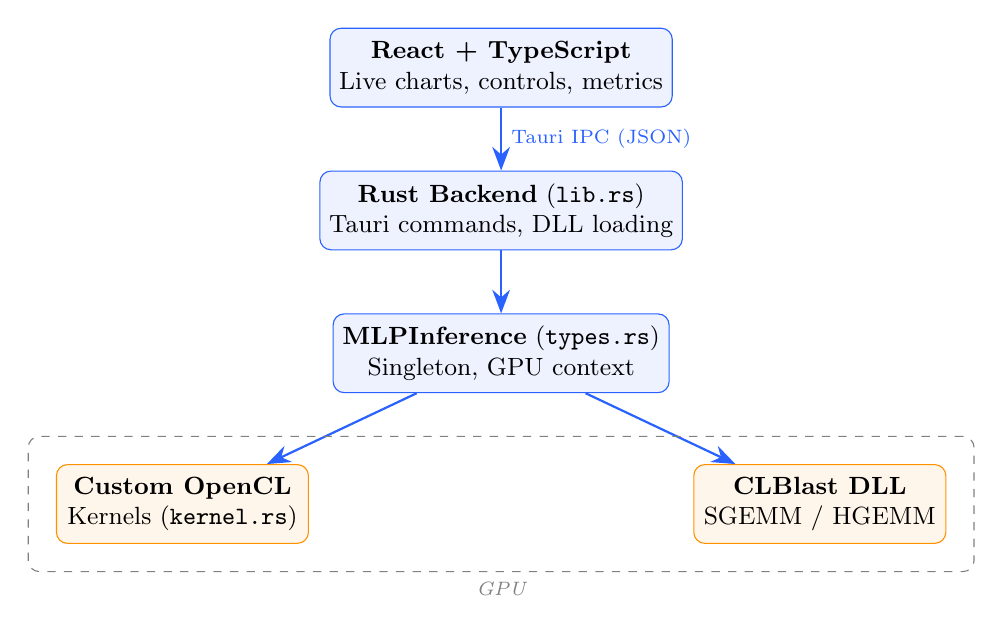
\begin{tikzpicture}[
		node distance=0.8cm and 1.2cm,
		box/.style={rectangle, draw=accentblue, fill=accentblue!8, rounded corners=4pt,
				minimum width=3.8cm, minimum height=1cm, align=center,
				font=\small},
		gpubox/.style={rectangle, draw=accentorange, fill=accentorange!8, rounded corners=4pt,
				minimum width=3.2cm, minimum height=1cm, align=center,
				font=\small},
		arr/.style={-{Stealth[length=3mm]}, thick, accentblue},
		]
		% Nodes
		\node[box] (frontend) {\textbf{React + TypeScript}\\Live charts, controls, metrics};
		\node[box, below=of frontend] (backend) {\textbf{Rust Backend} (\texttt{lib.rs})\\Tauri commands, DLL loading};
		\node[box, below=of backend] (mlp) {\textbf{MLPInference} (\texttt{types.rs})\\Singleton, GPU context};
		\node[gpubox, below left=0.9cm and 0.3cm of mlp] (opencl) {\textbf{Custom OpenCL}\\Kernels (\texttt{kernel.rs})};
		\node[gpubox, below right=0.9cm and 0.3cm of mlp] (clblast) {\textbf{CLBlast DLL}\\SGEMM / HGEMM};

		% Arrows
		\draw[arr] (frontend) -- node[right, font=\scriptsize] {Tauri IPC (JSON)} (backend);
		\draw[arr] (backend) -- (mlp);
		\draw[arr] (mlp) -- (opencl);
		\draw[arr] (mlp) -- (clblast);

		% Surrounding box
		\node[draw=gray, dashed, rounded corners, fit=(opencl)(clblast),
			inner sep=10pt, label={[font=\scriptsize\itshape, text=gray]below:GPU}] {};
	\end{tikzpicture}
\end{frame}

\begin{frame}{Backend File Structure}
	\begin{table}[h]
		\centering
		\renewcommand{\arraystretch}{1.3}
		\begin{tabularx}{0.88\textwidth}{lX}
			\toprule
			\textbf{File}      & \textbf{Responsibility}                                                                      \\
			\midrule
			\texttt{lib.rs}    & Tauri commands, CLBlast DLL embedding \& loading, device selection, FP16 helpers             \\
			\texttt{types.rs}  & All structs (\texttt{MLPInference}, \texttt{RoundData}, metrics) + all 6 inference functions \\
			\texttt{kernel.rs} & OpenCL C kernel source code (string constants, compiled at runtime)                          \\
			\texttt{logger.rs} & CSV export + PNG chart generation (\texttt{plotters}) for automatic logging                  \\
			\texttt{main.rs}   & Minimal entry point --- calls \texttt{lib::run()}                                            \\
			\bottomrule
		\end{tabularx}
	\end{table}
	\vspace{0.3cm}
	\textbf{Key design decisions:}
	\begin{itemize}
		\item \textbf{Singleton GPU context} --- avoids repeated OpenCL init ($\sim$200\,ms each)
		\item \textbf{Embedded DLL} --- \texttt{include\_bytes!} bakes CLBlast into the binary
		\item \textbf{Two-pass kernel design} --- Layer~1 and Layer~2 are separate dispatches
		\item \textbf{Pre-compiled helper kernels} --- bias/ReLU \& FP16 convert compiled once at startup
	\end{itemize}
\end{frame}

% ════════════════════════════════════════════════════════════════════
\section{Key Algorithms}
% ════════════════════════════════════════════════════════════════════

\begin{frame}{Two-Layer MLP Forward Pass}
	\begin{block}{Network Architecture}
		\[
			\underbrace{\mathbf{X}}_{64 \times N}
			\xrightarrow{\;\mathbf{W}_1^T + \mathbf{b}_1\;}
			\underbrace{\text{ReLU}(\mathbf{H})}_{64 \times N}
			\xrightarrow{\;\mathbf{W}_2^T + \mathbf{b}_2\;}
			\underbrace{\mathbf{Y}}_{64 \times N/2}
		\]
	\end{block}
	\vspace{0.2cm}
	\begin{itemize}
		\item \texttt{batch\_size} = 64 (fixed)
		\item \texttt{input\_size} = \texttt{hidden\_size} = \texttt{matrix\_size} (128 / 256 / 512 / 1024)
		\item \texttt{output\_size} = \texttt{matrix\_size} / 2
	\end{itemize}
	\vspace{0.3cm}
	\textbf{Layer 1:}\quad $\mathbf{H} = \text{ReLU}\!\big(\mathbf{X} \cdot \mathbf{W}_1^T + \mathbf{b}_1\big)$
	\\[4pt]
	\textbf{Layer 2:}\quad $\mathbf{Y} = \mathbf{H} \cdot \mathbf{W}_2^T + \mathbf{b}_2$
	\vspace{0.3cm}
	\begin{center}
		\small
		Same random $\mathbf{X}$ and deterministic $\mathbf{W}_1, \mathbf{W}_2, \mathbf{b}_1, \mathbf{b}_2$ for all 6 modes each round.
	\end{center}
\end{frame}

\begin{frame}{Row-Wise Weight Scaling (Mode 3)}
	\textbf{Problem:} Na\"ive FP16 conversion loses precision for large weight values.
	\vspace{0.3cm}

	\textbf{Solution:} Normalize each row so all values fit in $[-1, 1]$ (FP16's sweet spot):
	\vspace{0.2cm}

	\begin{block}{CPU Pre-processing}
		\[
			\text{scale}[h] = \max_i \big|\mathbf{W}[h][i]\big|
			\qquad\qquad
			\mathbf{W}_{\text{fp16}}[h] = \texttt{f32\_to\_f16}\!\left(\frac{\mathbf{W}[h]}{\text{scale}[h]}\right)
		\]
	\end{block}
	\vspace{0.1cm}
	\begin{block}{GPU Kernel --- recovering original magnitude}
		\[
			\text{sum} \mathrel{+}= \texttt{(float)}\,\text{input}[i] \;\times\; \texttt{(float)}\,\mathbf{W}_{\text{fp16}}[h][i] \;\times\; \text{scale}[h]
		\]
	\end{block}
	\vspace{0.3cm}
	\begin{itemize}
		\item All FP16 weight values are in $[-1.0,\;1.0]$ --- maximum representational density
		\item Hidden buffer kept as FP32 to avoid a second round of quantization error
		\item Small overhead: one extra multiply per element + storing the scale vector
	\end{itemize}
\end{frame}

\begin{frame}{CLBlast GEMM Integration (Modes 4--6)}
	\begin{block}{CLBlast SGEMM Call (per layer)}
		\lstinline|CLBlastSgemm(RowMajor, NoTrans, Trans, M, N, K, 1.0, A, B, 0.0, C)|
	\end{block}
	\vspace{0.2cm}
	\begin{itemize}
		\item \textbf{Transpose on $B$} (weights) avoids costly memory rearrangement
		\item BLAS has no concept of bias or ReLU $\Rightarrow$ separate helper kernels:
		      \begin{itemize}
			      \item \texttt{add\_bias\_relu} after Layer~1
			      \item \texttt{add\_bias} after Layer~2
		      \end{itemize}
	\end{itemize}
	\vspace{0.3cm}
	\textbf{CLBlast Mixed mode} additionally:
	\begin{enumerate}
		\item Uploads weights as FP16 (saves bandwidth)
		\item Runs \texttt{convert\_fp16\_to\_fp32} kernel \textbf{on GPU}
		\item Calls SGEMM in full FP32 $\Rightarrow$ near-FP32 accuracy
	\end{enumerate}
	\vspace{0.2cm}
	\begin{alertblock}{Auto-tuning}
		First GEMM call per matrix size triggers CLBlast's auto-tuner (1--3\,s).\\
		Solved by \texttt{warmup\_clblast()} before timing begins.
	\end{alertblock}
\end{frame}

% ════════════════════════════════════════════════════════════════════
\section{Metrics \& Methodology}
% ════════════════════════════════════════════════════════════════════

\begin{frame}{Performance Metrics}
	\renewcommand{\arraystretch}{1.4}
	\begin{table}[h]
		\centering
		\footnotesize
		\begin{tabularx}{0.95\textwidth}{l c X}
			\toprule
			\textbf{Metric} & \textbf{Unit}                                                                        & \textbf{Formula / Method} \\
			\midrule
			Execution Time
			                & ms
			                & Wall-clock: \texttt{Instant::now()} $\to$ \texttt{queue.finish()}                                                \\
			Throughput
			                & GFLOPS
			                & $\displaystyle\frac{\text{batch} \times \big[H(2I+1) + O(2H+1)\big]}{t \times 10^9}$                             \\
			Memory BW
			                & GB/s
			                & $\displaystyle\frac{\sum(\text{bytes read} + \text{bytes written})}{t \times 10^9}$                              \\
			Memory Footprint
			                & MB
			                & $\displaystyle\frac{\text{total GPU buffer bytes}}{1024^2}$                                                      \\
			Accuracy (MSE)
			                & ---
			                & $\displaystyle\frac{1}{N}\sum_{i}\big(\text{output}_i - \text{fp32\_ref}_i\big)^2$                               \\
			\bottomrule
		\end{tabularx}
	\end{table}
	\vspace{0.2cm}
	\begin{itemize}
		\item FP16 buffers count \textbf{2 bytes/elem}; FP32 buffers count \textbf{4 bytes/elem}
		\item FP32 and CLBlast FP32 always report MSE $= 0.0$ (they \emph{are} the reference)
		\item Timing excludes data generation and DLL loading
	\end{itemize}
\end{frame}

\begin{frame}{Evaluation Methodology}
	\begin{enumerate}
		\setlength{\itemsep}{0.4cm}
		\item \textbf{Shared data:} One \texttt{RoundData} struct (random input + deterministic weights) passed by reference to all 6 modes
		\item \textbf{Reference first:} FP32 always runs first; its output becomes the accuracy baseline
		\item \textbf{Warmup:} \texttt{warmup\_clblast()} fires untimed dummy GEMMs before measurement
		\item \textbf{Continuous benchmarking:} Self-chaining async loop runs all 6 modes back-to-back, updating 4 live charts per round
		\item \textbf{Adjustable workload:} Matrix size slider (128--1024) lets you study how problem size affects the tradeoffs
	\end{enumerate}
\end{frame}

\begin{frame}{Automatic Logging \& Plotting}
	Every \textbf{5 rounds}, the app automatically saves a full snapshot:
	\vspace{0.2cm}
	\begin{table}[h]
		\centering
		\renewcommand{\arraystretch}{1.25}
		\footnotesize
		\begin{tabularx}{0.88\textwidth}{lX}
			\toprule
			\textbf{File}                & \textbf{Contents}                                \\
			\midrule
			\texttt{metrics.csv}         & All metrics from round 1 to current, all 6 modes \\
			\texttt{execution\_time.png} & Line chart comparing execution time              \\
			\texttt{throughput.png}      & GFLOPS comparison                                \\
			\texttt{bandwidth.png}       & Memory bandwidth comparison                      \\
			\texttt{accuracy\_mse.png}   & Accuracy MSE vs FP32 baseline                    \\
			\bottomrule
		\end{tabularx}
	\end{table}
	\vspace{0.2cm}
	\textbf{Log path:} \texttt{parallel\_log/\{YYYY-MM-DD\_HH-MM-SS\}\_\{matrix\_size\}/}
	\vspace{0.3cm}
	\begin{itemize}
		\item New session folder created automatically when matrix size changes
		\item Charts generated server-side in Rust via the \textbf{plotters} crate
		\item Colors match the live dashboard (green / blue / purple / yellow / cyan / pink)
	\end{itemize}
\end{frame}

% ════════════════════════════════════════════════════════════════════
\section{Optimizations \& Challenges}
% ════════════════════════════════════════════════════════════════════

\begin{frame}{Optimization Techniques}
	\begin{table}[h]
		\centering
		\renewcommand{\arraystretch}{1.3}
		\footnotesize
		\begin{tabularx}{0.95\textwidth}{l l X}
			\toprule
			\textbf{Technique}           & \textbf{Where}             & \textbf{Effect}                                \\
			\midrule
			Two-pass kernel design       & Custom kernels             & Each hidden value computed once, not $O$ times \\
			CLBlast auto-tune warmup     & \texttt{warmup\_clblast()} & Prevents tuning latency in benchmarks          \\
			Pre-compiled OpenCL programs & Bias/ReLU + convert        & Saves $\sim$50\,ms per round                   \\
			Singleton GPU context        & \texttt{MLP\_INSTANCE}     & Avoids repeated OpenCL init ($\sim$200\,ms)    \\
			\texttt{spawn\_blocking}     & Tauri handlers             & Keeps UI thread responsive                     \\
			Single React dispatch        & \texttt{chartReducer}      & One re-render per round, not six               \\
			Embedded DLL                 & \texttt{include\_bytes!}   & Zero external dependencies                     \\
			\bottomrule
		\end{tabularx}
	\end{table}
\end{frame}

\begin{frame}{Challenges Encountered}
	\begin{columns}[T]
		\begin{column}{0.48\textwidth}
			\textbf{CLBlast auto-tuner latency}
			\begin{itemize}
				\item First GEMM call: 1--3\,s
				\item Solution: untimed warmup calls
			\end{itemize}
			\vspace{0.3cm}
			\textbf{FP16 in Rust}
			\begin{itemize}
				\item No native \texttt{f16} type
				\item Stored as \texttt{u16}, converted via \texttt{half} crate
				\item CLBlast \texttt{alpha}/\texttt{beta} also as \texttt{u16}
			\end{itemize}
		\end{column}
		\begin{column}{0.48\textwidth}
			\textbf{Thread safety of GPU state}
			\begin{itemize}
				\item Raw OpenCL handles not \texttt{Send+Sync}
				\item \texttt{unsafe impl} guarded by mutex
			\end{itemize}
			\vspace{0.3cm}
			\textbf{DLL distribution}
			\begin{itemize}
				\item External DLL is fragile
				\item Solution: \texttt{include\_bytes!} bakes DLL into \texttt{.exe}, extracted to \texttt{\%TEMP\%} at runtime
			\end{itemize}
		\end{column}
	\end{columns}
\end{frame}

% ════════════════════════════════════════════════════════════════════
\section{Results \& Analysis}
% ════════════════════════════════════════════════════════════════════

\begin{frame}{Expected Performance Results}
	\begin{center}
		\footnotesize
		\textit{Approximate relative values at} \texttt{matrix\_size = 512}, \texttt{batch\_size = 64}.
		\textit{Actual numbers vary by GPU.}
	\end{center}
	\vspace{0.1cm}
	\begin{table}[h]
		\centering
		\renewcommand{\arraystretch}{1.3}
		\begin{tabularx}{0.92\textwidth}{l c c c}
			\toprule
			\textbf{Mode}  & \textbf{Memory Footprint} & \textbf{Rel.\ Throughput} & \textbf{Accuracy MSE}   \\
			\midrule
			FP32           & 100\% (baseline)          & 1.0$\times$               & 0.0 (reference)         \\
			FP16           & $\sim$50\%                & 1.2--1.8$\times$          & Small, non-zero         \\
			FP16\,+\,Scale & $\sim$52\%                & 1.0--1.5$\times$          & \textbf{Less than FP16} \\
			CLBlast FP32   & $\sim$100\%               & 3--10$\times$             & 0.0                     \\
			CLBlast FP16   & $\sim$50\%                & 4--15$\times$             & Similar to FP16         \\
			CLBlast Mixed  & $\sim$150\%               & 2--8$\times$              & $\approx 0.0$           \\
			\bottomrule
		\end{tabularx}
	\end{table}
	\vspace{0.2cm}
	\begin{center}
		CLBlast advantages grow significantly at larger matrix sizes (512+).\\
		At \texttt{matrix\_size = 128}, custom kernels may be competitive due to CLBlast overhead.
	\end{center}
\end{frame}

\begin{frame}{Analysis}
	\begin{block}{Precision Format vs.\ Speed}
		FP16 kernels are faster due to \textbf{reduced memory bandwidth pressure}---each value is 2\,B instead of 4\,B. GPU cores run at similar speed for both.
	\end{block}
	\vspace{0.2cm}
	\begin{block}{BLAS vs.\ Custom Kernels}
		CLBlast is dramatically faster at large sizes: \textbf{tiled shared memory}, vectorized loads, and auto-tuned parameters vs.\ a simple inner loop.
	\end{block}
	\vspace{0.2cm}
	\begin{block}{Row-Wise Scaling Effect}
		FP16\,+\,Scale consistently shows \textbf{lower MSE} than plain FP16. Most visible when weights have high dynamic range. Small speed cost from extra multiply + FP32 hidden buffer.
	\end{block}
	\vspace{0.2cm}
	\begin{block}{CLBlast Mixed Tradeoff}
		Uses the most GPU memory (both FP16 + FP32 buffers), but achieves \textbf{near-FP32 accuracy} with FP16 upload bandwidth. Best when accuracy matters.
	\end{block}
\end{frame}

% ════════════════════════════════════════════════════════════════════
\section{Conclusions \& Future Work}
% ════════════════════════════════════════════════════════════════════

\begin{frame}{Conclusions}
	\begin{enumerate}
		\setlength{\itemsep}{0.35cm}
		\item \textbf{CLBlast is significantly faster} than hand-written kernels at medium-to-large sizes --- specialized BLAS optimizations cannot be matched by a simple loop.
		\item \textbf{FP16 halves memory footprint} and produces modest speedups, but accuracy loss is \textbf{real and measurable}.
		\item \textbf{Row-wise scaling meaningfully reduces FP16 error} by keeping values in FP16's most precise range. Accuracy benefit outweighs the small performance cost.
		\item \textbf{CLBlast Mixed offers near-FP32 accuracy at FP16 memory cost} --- the pragmatic production choice when accuracy cannot be compromised.
		\item \textbf{CLBlast auto-tuning is a one-time cost} that must be accounted for in benchmarks.
	\end{enumerate}
\end{frame}

\begin{frame}{Limitations}
	\begin{itemize}
		\setlength{\itemsep}{0.3cm}
		\item \textbf{Windows-only} --- CLBlast shipped as \texttt{.dll}; Linux/macOS would need \texttt{.so}/\texttt{.dylib}
		\item \textbf{Fixed batch size} (64) --- configurable batch would reveal more tradeoffs
		\item \textbf{No hardware counters} --- metrics are analytic, not measured from GPU perf counters
		\item \textbf{Auto-tuning per-session} --- CLBlast cache lost on app close
		\item \textbf{Two layers only} --- deeper networks may show different error accumulation behavior
	\end{itemize}
\end{frame}

\begin{frame}{Future Work}
	\begin{columns}[T]
		\begin{column}{0.48\textwidth}
			\begin{itemize}
				\setlength{\itemsep}{0.25cm}
				\item INT8 quantization for further memory reduction
				\item Deeper networks (4--8 layers) to study error accumulation
				\item Configurable batch size in the UI
				\item Cross-platform support (Linux/macOS)
			\end{itemize}
		\end{column}
		\begin{column}{0.48\textwidth}
			\begin{itemize}
				\setlength{\itemsep}{0.25cm}
				\item Hardware counter profiling for true bandwidth measurement
				\item BF16 (Brain Float 16) as an additional comparison point
				\item Transformer attention block to study mixed-precision in modern architectures
			\end{itemize}
		\end{column}
	\end{columns}
\end{frame}

\begin{frame}{Questions Addressed}
	\begin{description}
		\setlength{\itemsep}{0.3cm}
		\item[Objectives achieved?] Yes --- all 6 modes implemented, correct, and benchmarked fairly on the same data per round. Tradeoffs clearly visible in live dashboard.
		\item[Biggest bottleneck?] Custom kernels: \textbf{memory bandwidth}. CLBlast vs.\ custom: lack of \textbf{shared-memory tiling}.
		\item[vs.\ Expectations?] CLBlast delivered \textbf{larger speedups} than expected. Row-wise scaling delivered \textbf{more accuracy improvement} than expected at almost no throughput cost.
		\item[Do differently?] Use GPU hardware performance counters from the start; expose batch size as a UI parameter.
	\end{description}
\end{frame}

% ── End ─────────────────────────────────────────────────────────────

\begin{frame}{}
	\centering
	\vfill
	{\Huge\bfseries\color{accentblue} Thank You}
	\vspace{0.8cm}

	{\large Mixed-Precision Inference on GPUs}
	\vspace{0.3cm}

	{\small Built with \textbf{Rust} \(\cdot\) \textbf{OpenCL} \(\cdot\) \textbf{CLBlast} \(\cdot\) \textbf{Tauri} \(\cdot\) \textbf{React} \(\cdot\) \textbf{TypeScript}}
	\vspace{0.8cm}

	{\footnotesize\color{gray} GPU Computing Project --- Option 2: Mixed Precision with Row-Wise Scaling}
	\vfill
\end{frame}

\end{document}
